\documentclass[11pt]{article}

\usepackage{iftex}
\ifPDFTeX
  \usepackage[utf8]{inputenc}
  \usepackage[T1]{fontenc}
\fi
\usepackage[margin=1in]{geometry}
\usepackage{amsmath,amssymb,amsthm}
\usepackage{booktabs}
\usepackage{graphicx}
\usepackage{xcolor}
\usepackage{hyperref}
\usepackage{natbib}
\usepackage{microtype}
\usepackage{array}
\emergencystretch=3em
\hbadness=2000

\hypersetup{
  colorlinks=true,
  linkcolor=blue,
  citecolor=blue,
  urlcolor=blue
}

\newtheorem{proposition}{Proposition}
\newtheorem{lemma}{Lemma}
\newtheorem{definition}{Definition}

\title{\textbf{CREDO: Budgeted Channel Discovery and Selective Feature Acquisition for Imbalanced Prediction}}

\author{
  Wayne A. Satz, MD\\
  \small Department of Emergency Medicine, Lewis Katz School of Medicine at Temple University,\\
  \small Philadelphia, PA, USA \quad (\texttt{satzwa@temple.edu})
}

\date{November 2026}

\begin{document}

\maketitle

\begin{abstract}
Imbalanced prediction in clinical screening, industrial monitoring, and fraud detection is routinely addressed by resampling or reweighting a fixed baseline table $X_{\text{base}}$. When $X_{\text{base}}$ lacks conditional resolution among high-risk arrivals, improving precision requires identifying and selectively acquiring additional channels under explicit budgets. We present CREDO, a two-stage framework evaluated across 10 fixed-table benchmarks (50 splits), 9 multi-channel cohorts ($N = 10,000$ to $1,000,000$; 45 native-channel splits plus 40 echo-stress runs), and 7 failure-mode simulations. First, under Newton-stabilized gradient-boosted trees (\texttt{max\_delta\_step}$=1.0$) with natural-prevalence Platt calibration, SMOTE, ADASYN, copulas, EasyEnsemble, and RUSBoost yield no detectable AUPRC gains across 10 benchmarks ($p_{\text{NB}} \ge 0.068$, Holm $p \ge 0.88$), while small minority counts carry wide Wilson $95\%$ intervals. Second, an offset-anchored Horvitz--Thompson conditional log-likelihood gain estimator ($\hat{G}_m$) on a score-stratified case-cohort pilot improves over $X_{\text{base}}$ on $9/9$ native cohorts (Holm $p \le 0.018$ for AUPRC and $(\alpha,\delta)$-certified Neyman--Pearson sensitivity), matches $100\%$-row conditional discovery within $0.0009$ AUPRC on $8/9$ cohorts while saving $44.0\%$--$98.4\%$ of pilot accesses, and records $0.0\%$ false selection of injected echoes ($40/40$ runs vs.\ $30\%$--$50\%$ under marginal mutual information on large multi-table cohorts). Third, because class-conditional conformal coverage does not bound $\{1\}$ singleton precision under rarity (PPV $3.8\%$--$38.8\%$), upper-tail conformal acquisition achieves higher mean AUPRC than literal $\{0,1\}$ routing on $9/9$ cohorts (Holm $p \le 0.005$ on $5/9$) while tracking top-risk-$K$ ($p_2 \ge 0.215$) when Stage-1 risk stays below target precision.
\end{abstract}

\vspace{4pt}
\noindent\textbf{Keywords:} Imbalanced classification; case-cohort design; conditional mutual information; active feature acquisition; Mondrian conformal prediction; Neyman--Pearson classification.

\section{Introduction}

Prediction of rare adverse outcomes in clinical triage and hospital readmission screening \citep{strack2014impact}, physical equipment monitoring \citep{matzka2020explainable}, and financial or onboarding fraud detection \citep{dalpozzolo2014learned,jesus2022turning} operates under low event prevalence ($\pi = \mathbb{P}(Y=1) \in [10^{-3}, 0.20]$) alongside strict false-positive budgets ($\alpha_{\text{FPR}}$) or target positive predictive values ($q_{\text{target}}$) \citep{davis2006relationship,saito2015precision}. Standard machine-learning workflows typically attempt to improve rare-event performance on a fixed baseline feature table $X_{\text{base}}$ by modifying class proportions or loss weights via SMOTE \citep{chawla2002smote}, ADASYN \citep{he2008adasyn}, EasyEnsemble \citep{liu2009exploratory}, or RUSBoost \citep{seiffert2010rusboost}.

When two individuals share identical baseline intake covariates $X_{\text{base}} = x$ whose true conditional event probability satisfies $\eta_{\text{base}}(x) = \mathbb{P}(Y=1 \mid X_{\text{base}} = x) \ll q_{\text{target}}$, however, the limitation is informational rather than algorithmic. Overcoming baseline overlap requires answering two practical design questions under explicit measurement budgets \citep{covert2023learning,gadgil2024estimating,vonkleist2025evaluation}:
\begin{enumerate}
  \item \textbf{Budgeted Channel Discovery:} Given $M$ candidate Stage-2 feature channels $Z_1, \dots, Z_M$ (such as longitudinal utilization histories, relational credit-bureau tables, or secondary sensor suites) with acquisition costs $c_m > 0$, can a small, deliberately sampled pilot subset $\mathcal{P} \subset \mathcal{D}_{\text{train}}$ estimate conditional predictive utility above $X_{\text{base}}$ without measuring all $M$ channels across $100\%$ of training records---and without being misled by channels that merely repackage baseline risk?
  \item \textbf{Selective Runtime Acquisition:} Once a Stage-2 channel subset $\mathcal{S} \subseteq \{1,\dots,M\}$ is trained, how should a fixed deployment query budget $K$ be allocated across arriving instances, and when does class-conditional (Mondrian) conformal set construction \citep{lei2018distribution,sadinle2019least} add operational value beyond simple baseline-risk, uncertainty, or value-of-information (VOI) prioritization?
\end{enumerate}

Addressing these two questions rigorously requires separating population identities from finite-sample estimation and disentangling native database schemas from synthetic redundancy tests. In epidemiology, the case-cohort design of \citet{prentice1986casecohort} measures expensive covariates on all observed cases ($Y=1$) and a subcohort of controls ($Y=0$). Yet marginal mutual information $I(Y; Z_m)$---whether computed on the full cohort or on an unmatched case-control sample---rewards any channel correlated with baseline risk $X_{\text{base}}$. Conversely, conditioning only on a compressed scalar baseline score $S(X_{\text{base}})$ can miss pure $[X_{\text{base}}, Z_m]$ interactions, while aggressive collinearity penalties risk discarding correlated channels that still carry informative conditional residuals. Similarly, at deployment, two-stage conformal cascades designed for balanced classification query Stage-2 features strictly on the multi-label ambiguity region $\mathcal{C}_1(x) = \{0,1\}$ while accepting singleton sets $\{1\}$ and $\{0\}$ unverified. Under severe class imbalance, class-conditional coverage $\mathbb{P}(0 \in \mathcal{C}_1(X) \mid Y=0) \ge 1 - \alpha_0$ bounds the false-positive rate of $\{1\}$ singletons only by $\alpha_0$, which permits low singleton precision whenever $\pi \ll \alpha_0$ unless the Stage-1 score achieves near-perfect tail separation.

In this paper, we introduce \textbf{CREDO} (\emph{Calibrated Receipt-Repaired Evidence Discovery and Orchestration}) and evaluate both its strengths and its exact failure modes across \textbf{CREDO-Bench}. Rather than claiming universal optimality, we establish precise population lemmas, finite-sample distribution-free operating-point guarantees, and controlled single-factor empirical comparisons:
\begin{itemize}
  \item \textbf{Fixed-Table Baseline Evaluation and Uncertainty Accounting (Section~\ref{sec:fixed_table}, Lemma~\ref{lem:prior_shift}):} At the population level, shifting class priors while preserving class-conditional distributions is strictly rank-preserving \citep{elkan2001foundations}. Because finite-sample resampling algorithms alter empirical class-conditional distributions and estimator variance, we test empirically whether SMOTE, ADASYN, copula augmentation, EasyEnsemble, or RUSBoost improve out-of-sample AUPRC over Newton-stabilized, natural-prevalence Platt-calibrated LightGBM across 10 public fixed-table datasets ($50$ four-way splits), paired with exact Wilson $95\%$ operating-point sensitivity intervals \citep{wilson1927probable}.
  \item \textbf{Horvitz--Thompson Stratified-Pilot Conditional Log-Likelihood Gain (Section~\ref{sec:discovery}, Lemma~\ref{lem:ht_cmi}):} We construct a baseline-score-stratified case-cohort pilot with strictly positive known stratum inclusion probabilities $\pi_{0,b} = n_{0,b}/N_{0,b} > 0$ and exact Horvitz--Thompson weights summing to $N_0$, and score each candidate channel via cross-fitted offset-anchored gradient-boosted conditional log-likelihood gain $\hat{G}_m$ over $[X_{\text{base}}, Z_m]$. We evaluate native-only channels (including an unrestricted all-native-channels GBDT reference and explicit discovery + training + deployment access accounting) separately from injected baseline-echo stress tests and downstream ensemble complexity ablations.
  \item \textbf{Conformal Singleton Precision Analysis and Six-Policy Runtime Routing (Section~\ref{sec:routing}, Proposition~\ref{prop:singleton}):} We characterize when Mondrian $\{1\}$ singletons fail precision targets under low prevalence, implement distribution-free $(\alpha,\delta)$ Neyman--Pearson thresholds via strict-inequality order statistics \citep{tong2018neyman}, and benchmark CREDO upper-tail conformal acquisition at identical query budgets against five comparators: literal $\{0,1\}$ conformal ambiguity routing, top-risk-$K$ prioritization, uncertainty-$K$ routing, decision-focused VOI-$K$ loss-reduction routing, and random-$K$ routing, supplemented by 7 adversarial simulations that expose exact failure boundaries (including pure XOR interactions, Stage-1 underfitting, irreducible top-risk pockets where VOI-$K$ and literal $\{0,1\}$ dominate upper-tail routing, and temporal covariate drift \citep{barber2023conformal}).
\end{itemize}

\subsection{Motivating Clinical Admission-Time Screening Problem}
\label{sec:clinical_motivation}

To ground the methodology in a concrete clinical workflow, consider admission-time screening for unplanned $<30$-day hospital readmission on \texttt{UCI Diabetes 130-US Hospitals} \citep{strack2014impact}. Out of $101,766$ raw inpatient encounters across $71,518$ unique patients, encounters ending in inpatient death or hospice discharge (\texttt{discharge\_disposition\_id} $\in \{11, 13, 14, 19, 20, 21\}$; $2,423$ encounters, including $43$ carrying a recorded \texttt{<30} code) cannot enter the post-discharge readmission risk set and are excluded upfront using disposition codes alone, independent of $Y$, leaving $99,343$ eligible encounters ($\pi = 11.39\%$).

At the moment of hospital admission, only seven inexpensive intake variables reside in $X_{\text{base}}$: patient age bucket, gender, race, admission type, admission source, primary payer code, and weight documentation flag. Variables accumulated during or at the end of the stay---such as length of stay (\texttt{time\_in\_hospital}), cumulative inpatient laboratory and procedure counts, historical outpatient/emergency/inpatient utilization lookups, medication changes, diagnostic comorbidity coding, HbA1c/glucose results, and discharge care-transition routing---are unavailable at admission intake and represent candidate Stage-2 channels in a retrospective feature-access simulation \citep{vonkleist2025evaluation}. Two patients arriving through the emergency department with identical intake fields $X_{\text{base}} = x$ cannot be separated by resampling $X_{\text{base}}$. Meanwhile, auditing all six candidate EHR and utilization channels across $100\%$ of training charts during development or $100\%$ of arrivals at deployment incurs substantial chart-abstraction or interface burden, motivating budgeted pilot discovery followed by selective Stage-2 retrieval.

\section{Statistical Framework and Methodology}

\subsection{Problem Formulation, Eligibility, and Strict Chronological/Grouped Splitting}
\label{sec:splits}

Let $(X_{\text{base}}, Z_1, \dots, Z_M, Y, \tilde{Y})$ denote an observational or simulated screening cohort where $X_{\text{base}} \in \mathcal{X}$ is observed at baseline for all eligible arrivals, $Z_m \in \mathcal{Z}_m$ ($m=1,\dots,M$) are candidate Stage-2 feature channels with per-instance acquisition costs $c_m > 0$ and discovery pilot budget $\sum_{m \in \mathcal{S}} c_m \le B$, $Y \in \{0,1\}$ is the target rare outcome ($\pi = \mathbb{P}(Y=1) < 0.5$), and $\tilde{Y} \in \{0,1\}$ is the recorded outcome receipt when ascertainment is incomplete \citep{elkan2008learning,lakkaraju2017selective}. An operational decision contract $\mathcal{K} = (q_{\text{target}}, \alpha_{\text{FPR}}, C_{\text{FP}}, C_{\text{FN}}, C_{\text{graded}})$ specifies target precision $q_{\text{target}}$, false-positive rate ceiling $\alpha_{\text{FPR}}$, false-positive cost $C_{\text{FP}}$, false-negative cost $C_{\text{FN}}$, and optional reversible review cost $C_{\text{graded}} < C_{\text{FP}}$.

\textbf{Upfront Outcome-Independent Eligibility:} Whenever a cohort contains structurally ineligible records (e.g., inpatient death/hospice discharges in \texttt{UCI Diabetes 130-US}, or accounts already delinquent at baseline month 6 with \texttt{PAY\_6} $> 0$ in \texttt{UCI Taiwan Credit}, where $3,079$ of $30,000$ accounts including $1,611$ defaults are excluded upfront), eligibility masks are defined strictly from pre-outcome or administrative disposition fields \emph{prior} to data splitting and without inspecting $Y$. Every exclusion count (total and $Y=1$) is logged in the campaign audit manifest.

\textbf{Four-Way Split and Causal Cross-Fitting Protocol:} Each eligible cohort is partitioned into $\mathcal{D}_{\text{train}}$ ($55\%$), $\mathcal{D}_{\text{cal}}$ ($15\%$), $\mathcal{D}_{\text{val}}$ ($15\%$), and $\mathcal{D}_{\text{test}}$ ($15\%$) with SHA-256 index verification under dataset-specific dependency constraints:
\begin{enumerate}
  \item \textbf{Entity-Grouped Splits:} When repeated entity identifiers $G$ exist without a global calendar clock (\texttt{UCI Diabetes 130-US}, $71,518$ patients), group-disjoint splitting ensures zero patient overlap across all four partitions.
  \item \textbf{Strict Forward Chronological Splits and Expanding-Block Cross-Fitting:} On timestamped cohorts (\texttt{ULB Credit Card}, \texttt{IEEE-CIS}, \texttt{NeurIPS BAF}), $\mathcal{D}_{\text{train}}$, $\mathcal{D}_{\text{cal}}$, $\mathcal{D}_{\text{val}}$, and $\mathcal{D}_{\text{test}}$ are ordered strictly forward in time across 5 staggered windows or disjoint future eras. Inside $\mathcal{D}_{\text{train}}$, out-of-fold (OOF) nuisance predictions are generated exclusively via causal expanding-block cross-validation satisfying $\max_{i \in \text{train}_k} T_i < \min_{j \in \text{val}_k} T_j$ on every fold $k$. The earliest chronological burn-in block (which has no prior training history) is excluded via an explicit causal mask (\texttt{oof\_valid\_mask}) from OOF-dependent selection rather than predicted backward from future blocks or silently replaced by random CV. When both $G$ and $T$ are present, forward chronological splits purge any training entity reappearing in later folds.
  \item \textbf{Stratified Splits:} On cross-sectional tables without timestamps or repeated entity IDs (Tier-1 datasets, \texttt{Gate 0.5}, \texttt{UCI AI4I}, \texttt{UCI Taiwan Credit}, \texttt{Scania APS}, \texttt{Home Credit}), four-way splits stratify on $Y$, and all relational child-table aggregations ($20.8\text{M}$ rows across 6 auxiliary tables in \texttt{Home Credit}) and stateful feature compilers \citep{scheffer2009early} are fit strictly on $\mathcal{D}_{\text{train}}$.
\end{enumerate}

\subsection{Stabilized Fixed-Table Baselines and Exploratory Bottleneck Diagnostics}
\label{sec:fixed_table}

In binary log-loss gradient boosting, Newton--Raphson leaf steps take the form $\sum g_i / \sum h_i$ with gradient $g_i = \hat{p}_i - y_i$ and Hessian $h_i = \hat{p}_i(1-\hat{p}_i)$. Under rare prevalence, leaves with $\hat{p}_i \ll 10^{-2}$ have near-zero Hessians, causing unclipped leaf updates to overshoot unless regularized. Our baseline fixed-table model bounds leaf step magnitude via \texttt{max\_delta\_step}$=1.0$ in regularized LightGBM \citep{ke2017lightgbm} and applies monotonic logit-scale Platt calibration on natural-prevalence $\mathcal{D}_{\text{cal}}$ ($\varepsilon_{\text{clip}} = 10^{-15}$).

\begin{lemma}[Prior-Shift Invariance of Population Oracle Ranking]
\label{lem:prior_shift}
Let $\eta_{\text{base}}(x) = \mathbb{P}(Y=1 \mid X_{\text{base}}=x)$ denote the population posterior under $(\mathcal{X}, \mathbb{P})$ with class prior $\pi \in (0,1)$. Any prior-shift or cost-reweighting operator \citep{elkan2001foundations} that changes the effective prior from $\pi$ to $\tilde{\pi} \in (0,1)$ while leaving the class-conditional distributions $\mathbb{P}(X_{\text{base}} \mid Y=1)$ and $\mathbb{P}(X_{\text{base}} \mid Y=0)$ unchanged induces the Bayes-optimal posterior
\begin{equation}
  \tilde{\eta}(x) = \frac{\gamma \eta_{\text{base}}(x)}{\gamma \eta_{\text{base}}(x) + 1 - \eta_{\text{base}}(x)}, \qquad \gamma = \frac{\tilde{\pi}(1-\pi)}{\pi(1-\tilde{\pi})} > 0.
\end{equation}
Because $u \mapsto \gamma u / (\gamma u + 1 - u)$ is strictly increasing on $[0,1]$, $\tilde{\eta}(X_{\text{base}})$ induces the same population ROC and Precision--Recall curves as $\eta_{\text{base}}(X_{\text{base}})$ while distorting probability calibration on natural prevalence whenever $\tilde{\pi} \ne \pi$. Furthermore, the additional log-likelihood ratio beyond $\eta_{\text{base}}(x)$ needed to reach posterior precision $q_{\text{target}}$ is the \emph{instance log-evidence deficit}
\begin{equation}
  D_q(x) = \max\!\left\{0,\; \operatorname{logit}(q_{\text{target}}) - \operatorname{logit}(\eta_{\text{base}}(x))\right\}.
\end{equation}
\end{lemma}

\textbf{Scope of Lemma~\ref{lem:prior_shift}:} Lemma~\ref{lem:prior_shift} is a population statement about pure prior shifts; it does \emph{not} imply that finite-sample resampling is universally inert. Synthetic interpolation (SMOTE, ADASYN, copulas) modifies empirical class-conditional feature distributions, and bagged undersampling (EasyEnsemble, RUSBoost) alters tree split geometries and variance. Whether those finite-sample perturbations improve or degrade out-of-sample AUPRC relative to a step-stabilized, calibrated GBDT is therefore an empirical question tested in Section~\ref{sec:res_tier1}.

\textbf{Exploratory Bottleneck Diagnostic Panel:} Alongside baseline training, CREDO reports four descriptive diagnostics (explicitly treated as exploratory heuristics rather than universal Bayes bounds): (i) both the prespecified planning sensitivity half-width at $80\%$ sensitivity ($1.96\sqrt{0.16/n_{+,\text{test}}}$) and the exact observed Binomial Wilson $95\%$ sensitivity confidence interval \citep{wilson1927probable} at the test operating point; (ii) an empirical outcome-receipt discrepancy index ($\text{ADI}$) when auxiliary ascertainment proxies exist on $\mathcal{D}_{\text{train}}$; (iii) Expected Calibration Error (ECE) before versus after Platt calibration; and (iv) an out-of-sample standardized $k$-NN local label purity check from $\mathcal{D}_{\text{train}}$ to $\mathcal{D}_{\text{val}}$.

\subsection{Horvitz--Thompson Stratified-Pilot Conditional Log-Likelihood Gain}
\label{sec:discovery}

When baseline covariates leave substantial overlap among high-risk arrivals, we wish to select a subset of Stage-2 channels $\mathcal{S} \subseteq \{1,\dots,M\}$ under budget $\sum_{m \in \mathcal{S}} c_m \le B$ without measuring every candidate channel across all $N_{\text{train}}$ training records. Let $\hat{\eta}_{\text{base}}(X_{\text{base}})$ denote the leak-free OOF baseline probability on the valid causal training subset of size $N = N_+ + N_0$. Partition the $N$ training records into $B_{\text{strata}}$ quantile bins of $\operatorname{logit}(\hat{\eta}_{\text{base}}(X_{\text{base}}))$, containing $N_{+,b}$ cases and $N_{0,b}$ controls in bin $b$.

\textbf{Known-Probability Stratified Case-Cohort Pilot:} Our pilot $\mathcal{P} = \mathcal{P}_+ \cup \mathcal{P}_0$ includes all valid training cases ($\mathcal{P}_+$, inclusion probability $\pi_{+,i} = 1$, weight $w_i = 1$) and draws $n_0 = \min(N_0, m(\pi) N_+)$ controls without replacement across the $B_{\text{strata}}$ baseline score bins using a variance-controlled hybrid allocation: $35\%$ proportional to control bin size $N_{0,b}$ (guaranteeing a strictly positive inclusion floor in every bin) and $65\%$ proportional to case bin count $N_{+,b}$ (concentrating controls in the high-risk baseline strata where cases reside), subject to $1 \le n_{0,b} \le N_{0,b}$. Each sampled control $i \in \mathcal{P}_0$ in bin $b$ has exact known inclusion probability $\pi_{0,b} = n_{0,b}/N_{0,b} > 0$ and exact Horvitz--Thompson (HT) inverse-probability weight $w_i = N_{0,b}/n_{0,b}$ \citep{horvitz1952generalization}, satisfying $\sum_{i \in \mathcal{P}_0} w_i = \sum_{b=1}^{B_{\text{strata}}} n_{0,b}(N_{0,b}/n_{0,b}) = N_0$ identically \citep{prentice1986casecohort}.

\textbf{Offset-Anchored Conditional Log-Likelihood Gain ($\hat{G}_m$):} To evaluate each candidate channel $Z_m$ on $\mathcal{P}$ without collapsing $X_{\text{base}}$ to a scalar summary (which would miss pure $[X_{\text{base}}, Z_m]$ interactions) and without heuristic collinearity penalties, we fit two shallow, identically regularized GBDT models across identical leak-free pilot CV folds using HT sample weights $w_i$ and baseline log-odds offset $\texttt{init\_score}_i = \operatorname{logit}(\hat{\eta}_{\text{base}}(X_{\text{base},i}))$: a baseline-only pilot model $\hat{p}_{\text{base},\mathcal{P}}(X_{\text{base}})$ and an augmented model $\hat{p}_{m,\mathcal{P}}(X_{\text{base}}, Z_m)$, each calibrated fold-internally via HT-weighted logistic regression on its raw margin. Denoting binary cross-entropy by $\ell(y, p) = -[y \log p + (1-y)\log(1-p)]$, the Horvitz--Thompson conditional log-likelihood gain estimator is
\begin{equation}
  \label{eq:ht_gain}
  \hat{G}_m = \frac{1}{N} \sum_{i \in \mathcal{P}} w_i \left[\ell\!\left(Y_i, \hat{p}_{\text{base},\mathcal{P}}(X_{\text{base},i})\right) - \ell\!\left(Y_i, \hat{p}_{m,\mathcal{P}}(X_{\text{base},i}, Z_{m,i})\right)\right]_+.
\end{equation}
Channels with $\hat{G}_m > 0$ are selected greedily by cost-normalized utility $\hat{G}_m / c_m$ up to budget $B$.

\begin{lemma}[Population Conditional Mutual Information Target and Horvitz--Thompson Unbiasedness]
\label{lem:ht_cmi}
Let $\eta_{\text{base}}(x) = \mathbb{P}(Y=1 \mid X_{\text{base}}=x)$ and $\eta_m(x, z) = \mathbb{P}(Y=1 \mid X_{\text{base}}=x, Z_m=z)$ denote the true population posteriors, and let $g_m(x, z, y) = \ell(y, \eta_{\text{base}}(x)) - \ell(y, \eta_m(x, z))$. Then:
\begin{enumerate}
  \item At the population posteriors, $\mathbb{E}[g_m(X_{\text{base}}, Z_m, Y)] = I(Y; Z_m \mid X_{\text{base}}) \ge 0$ \citep{covert2023learning,gadgil2024estimating}, with equality $I(Y; Z_m \mid X_{\text{base}}) = 0$ if and only if $Y \perp Z_m \mid X_{\text{base}}$ (which holds for any baseline echo $Z_{\text{red}} = h(X_{\text{base}}, \varepsilon)$ with $\varepsilon \perp Y \mid X_{\text{base}}$), whereas $I(Y; Z_m \mid X_{\text{base}}) > 0$ both for pure interaction channels ($I(Y; Z_m) = 0$ but $I(Y; Z_m \mid X_{\text{base}}) > 0$) and for baseline-correlated channels carrying informative conditional residuals.
  \item Under stratified case-cohort sampling with $\pi_{+,i} = 1$ and $\pi_{0,b} = n_{0,b}/N_{0,b} > 0$, the Horvitz--Thompson functional $\frac{1}{N}\sum_{i \in \mathcal{P}} w_i \psi_i$ is design-unbiased for the full-cohort empirical average $\frac{1}{N}\sum_{i=1}^{N} \psi_i$ for any fixed per-record loss difference $\psi_i$: $\mathbb{E}_{\mathcal{P}}\!\left[\frac{1}{N}\sum_{i \in \mathcal{P}} w_i \psi_i \,\middle|\, \mathcal{D}_{\text{train}}\right] = \frac{1}{N}\sum_{i=1}^{N} \psi_i$.
\end{enumerate}
\end{lemma}

\textbf{Prespecified Matching-Ratio Heuristic and Failure Conditions:} Motivated by the classical two-sample stratum relative efficiency $m/(m+1)$ ($80\%$ at $m=4$) \citep{prentice1986casecohort}, we prespecify the control-to-case ratio heuristic $m(\pi) = 2$ for $\pi \ge 0.10$ (limiting pilot size when cases are common), $m(\pi) = 4$ for $\pi \in [0.005, 0.10)$, and $m(\pi) = 8$ for ultra-rare $\pi < 0.005$ (stabilizing small case counts while still sampling $<2\%$ of records); we test sensitivity across $m \in \{1,2,4,8,16\}$ directly in Simulation~5. Importantly, Lemma~\ref{lem:ht_cmi}(1) holds at the true conditional risk $\eta_{\text{base}}(x)$: if the Stage-1 model severely misspecifies nonlinear structure in $X_{\text{base}}$, a nonlinear transformation $h(X_{\text{base}})$ can still yield apparent empirical gain $\hat{G}_m > 0$ (verified in Simulation~4).

\textbf{Downstream Estimator Complexity and Total Access Accounting:} Our primary downstream estimator (\textbf{Arm A5}) trains a \emph{single} stabilized, Platt-calibrated GBDT on $[X_{\text{base}}, Z_{\mathcal{S}}]$ across $\mathcal{D}_{\text{train}}$, isolating channel discovery from ensemble complexity. As secondary architectural ablations, we also evaluate an equal-capacity 6-learner heterogeneous ensemble (\textbf{Arm A6e}), a separate-branch orthogonal log-odds lattice (\textbf{Arm A6}), and a Platt-recalibrated hybrid lattice (\textbf{Arm A7}) weighted by the calibration negative-tail coincidence ratio $\kappa_0$ computed via circular index shifts on $Y=0$. Furthermore, because selective discovery measures all $M$ candidate channels on the pilot $\mathcal{P}$ and then measures only the selected subset $\mathcal{S}$ on non-pilot training/calibration records and queried test arrivals, we explicitly audit all three components of channel access volume:
\begin{equation}
  C_{\text{total}} = \underbrace{|\mathcal{P}|\, M}_{\text{pilot discovery}} + \underbrace{(|\mathcal{D}_{\text{train}} \setminus \mathcal{P}| + |\mathcal{D}_{\text{cal}}| + |\mathcal{D}_{\text{val}}|)\, |\mathcal{S}|}_{\text{selected-channel model fitting \& calibration}} + \underbrace{K_{\text{query}}\, |\mathcal{S}|}_{\text{selective deployment}}.
\end{equation}

\subsection{Conformal Singleton Precision, Certified NP Thresholds, and Runtime Routing}
\label{sec:routing}

At deployment, Stage 1 produces calibrated baseline risk $\hat{p}_1(x)$ on $X_{\text{base}}$. Using $\mathcal{D}_{\text{cal}}$, Mondrian conformal prediction \citep{lei2018distribution,sadinle2019least} constructs prediction sets $\mathcal{C}_1(x) \subseteq \{0,1\}$ at class-conditional miscoverage targets $(\alpha_0, \alpha_1)$ via finite-sample order statistics $\hat{q}_{1-\alpha_0}^{(0)}$ on calibration negatives ($Y=0$) and $\hat{q}_{1-\alpha_1}^{(1)}$ on calibration positives ($Y=1$):
\begin{equation}
  0 \in \mathcal{C}_1(x) \iff \hat{p}_1(x) \le \hat{q}_{1-\alpha_0}^{(0)}, \qquad 1 \in \mathcal{C}_1(x) \iff 1 - \hat{p}_1(x) \le \hat{q}_{1-\alpha_1}^{(1)}.
\end{equation}

\begin{proposition}[Class-Conditional Coverage Does Not Guarantee Positive-Singleton Precision]
\label{prop:singleton}
Let $\mathcal{S}_{\{1\}} = \{x : \mathcal{C}_1(x) = \{1\}\}$ be a non-empty positive singleton region with class-conditional capture rates $\gamma_1 = \mathbb{P}(X \in \mathcal{S}_{\{1\}} \mid Y=1) \le 1 - \alpha_1$ and $\gamma_0 = \mathbb{P}(X \in \mathcal{S}_{\{1\}} \mid Y=0) \le \alpha_0$. By Bayes' rule, the precision inside $\mathcal{S}_{\{1\}}$ is
\begin{equation}
  \operatorname{PPV}(\mathcal{S}_{\{1\}}) = \frac{\pi \gamma_1}{\pi \gamma_1 + (1-\pi)\gamma_0},
\end{equation}
which falls strictly below $q_{\text{target}}$ whenever $\pi < q_{\text{target}}\gamma_0 / [q_{\text{target}}\gamma_0 + (1-q_{\text{target}})\gamma_1]$. Because Mondrian calibration constrains only the upper bound $\gamma_0 \le \alpha_0$, two distinct regimes arise at $\pi = 0.01, \alpha_0 = 0.05, \gamma_1 = 0.95$: if the threshold binds near the nominal boundary ($\gamma_0 = 0.05$), $\operatorname{PPV}(\mathcal{S}_{\{1\}}) = 16.1\%$ (dominated by false positives), whereas if Stage 1 achieves extreme tail separation ($\gamma_0 = 10^{-4} \ll \alpha_0$), $\operatorname{PPV}(\mathcal{S}_{\{1\}}) = 99.0\%$. Thus class-conditional coverage alone cannot certify singleton precision without inspecting $\hat{p}_1(x)$ relative to $q_{\text{target}}$.
\end{proposition}

\textbf{Six Equal-Budget Runtime Routing Policies:} Given the query budget $K = |\mathcal{Q}_{\text{CREDO}}|$ induced by CREDO's upper-tail evidence-deficit rule $\mathcal{Q}_{\text{CREDO}} = \{x : 1 \in \mathcal{C}_1(x) \text{ and } \hat{p}_1(x) < \max(q_{\text{target}}, 0.85)\}$, we compare six policies at the \emph{exact same} Stage-2 query count $K$:
\begin{enumerate}
  \item \textbf{CREDO Upper-Tail ($\mathcal{Q}_{\text{CREDO}}$):} Queries instances with $1 \in \mathcal{C}_1(x)$ whose Stage-1 probability has not yet certified $\max(q_{\text{target}}, 0.85)$; unqueried $\{0\}$ singletons are assigned hard negative decisions.
  \item \textbf{Literal Conformal Ambiguity ($\{0,1\}$):} Queries $\mathcal{M}_{01} = \{x : \mathcal{C}_1(x) = \{0,1\}\}$ first; if $|\mathcal{M}_{01}| > K$, selects the $K$ instances closest to the boundary; if $|\mathcal{M}_{01}| < K$, pads from $\{0\}$ singletons closest to $\hat{q}_{1-\alpha_0}^{(0)}$---never artificially skipping top-risk records when $\mathcal{S}_{\{1\}}$ is empty.
  \item \textbf{Top-Risk-$K$:} Queries the $K$ instances with highest Stage-1 risk $\hat{p}_1(x)$ directly, testing whether conformal machinery adds ranking value beyond simple risk prioritization.
  \item \textbf{Uncertainty-$K$:} Queries the $K$ instances minimizing $|\hat{p}_1(x) - \tau^*|$, where $\tau^* = C_{\text{FP}}/(C_{\text{FP}} + C_{\text{FN}})$ is the Bayes cost-optimal decision threshold.
  \item \textbf{Estimated VOI-$K$ (Expected Bayes Loss Reduction):} Queries the $K$ instances maximizing estimated Bayes action-loss reduction $\widehat{\operatorname{VOI}}(x) = \ell_{\mathcal{K}}(\hat{p}_1(x)) - \mathbb{E}[\ell_{\mathcal{K}}(\hat{p}_2) \mid \hat{p}_1(x)]$, where $\ell_{\mathcal{K}}(p) = \min\{p C_{\text{FN}}, (1-p) C_{\text{FP}}\}$ and the conditional posterior variance is fit on $\mathcal{D}_{\text{cal}}$.
  \item \textbf{Random-$K$:} Queries $K$ instances uniformly at random without replacement.
\end{enumerate}
Notice an immediate structural consequence of $\mathcal{Q}_{\text{CREDO}}$: whenever $\max_x \hat{p}_1(x) < \max(q_{\text{target}}, 0.85)$ across test arrivals, the upper probability cutoff never binds, so $\mathcal{Q}_{\text{CREDO}}$ reduces to a baseline-risk threshold $\{1 \in \mathcal{C}_1(x)\}$ whose ordering coincides with \textbf{Top-Risk-$K$} (differing only in that Mondrian calibration determines the query count $K$). Conversely, if a high-risk pocket already satisfies $\hat{p}_1(x) > \tau^*$ with zero Stage-2 uncertainty while a mid-risk pocket near $\tau^*$ resolves cleanly at Stage 2, \textbf{VOI-$K$} and \textbf{Literal $\{0,1\}$} will outperform both \textbf{Top-Risk-$K$} and \textbf{CREDO Upper-Tail} (demonstrated in Simulation~6). Moreover, Mondrian coverage guarantees assume exchangeability between $\mathcal{D}_{\text{cal}}$ and $\mathcal{D}_{\text{test}}$ and can degrade under temporal drift \citep{barber2023conformal} (quantified in Simulation~7).

\textbf{Distribution-Free $(\alpha,\delta)$ Neyman--Pearson Operating Points:} For hard binary screening at false-positive budget $\alpha = \alpha_{\text{FPR}}$ with confidence $1-\delta$ ($\delta = 0.05$), we implement the exact Binomial order-statistic threshold of \citet{tong2018neyman} on the $m = |\mathcal{D}_{\text{cal},0}|$ negative calibration scores $S_{(1)} \le \dots \le S_{(m)}$, selecting the smallest $r \in \{1,\dots,m\}$ satisfying $\sum_{j=r}^{m} \binom{m}{j}(1-\alpha)^j \alpha^{m-j} \le \delta$ (certified feasible iff $(1-\alpha)^m \le \delta$) and classifying test instances via the \emph{strict} inequality $S(x) > S_{(r)}$. As proved in Appendix~\ref{app:proofs}, strict inequality ensures that discrete or tied negative scores never exceed false-positive rate $\alpha$ with probability at least $1-\delta$ under exchangeability.

\subsection{Statistical Inference}

To account for training-set overlap across $K_{\text{seed}}=5$ repeated four-way splits, we apply the conservative Nadeau--Bengio variance correction \citep{nadeau2003inference}:
\begin{equation}
  \text{SE}_{\text{NB}} = \sqrt{\left(\frac{1}{K_{\text{seed}}} + \rho_{\text{overlap}} \frac{n_{\text{test}}}{n_{\text{train}}}\right) s_\Delta^2},
\end{equation}
setting $\rho_{\text{overlap}} = 1$ on all real observational cohorts (including staggered chronological windows where training histories partially overlap, and $\rho_{\text{overlap}} = 0$ only on independently simulated \texttt{Gate 0.5} populations), paired with step-down Holm--Bonferroni family-wise error rate (FWER) adjustment \citep{holm1979simple} rather than weaker false-discovery-rate control \citep{benjamini1995controlling} across every primary hypothesis family.

\subsection{Ethics Statement}

This study performs retrospective computational and statistical analyses solely on publicly available, de-identified benchmark datasets \citep{strack2014impact,yeh2009comparisons,matzka2020explainable,dalpozzolo2014learned,jesus2022turning}. No human subjects were recruited or intervened upon, no identifiable private health information was accessed, and no clinical care recommendations are made; this work is exempt from IRB review and informed consent under 45 CFR 46.104(d)(4).

\subsection{AI-Assisted Workflows and Reproducibility}

Portions of the computational workflow---specifically Python benchmark scaffolding, counterexample regression tests, and LaTeX formatting---were conducted using Google Antigravity powered by Gemini 3.1 Pro with the Google DeepMind Science Plugin (v1.4.0). Zero generative AI calls occur inside the CREDO algorithms, which execute as deterministic numerical software. All generated code, dataset loaders, bibliographic citations, statistical analyses, and scientific conclusions were independently executed and verified by the human author, who takes full responsibility for the integrity of this work.

\section{Empirical Results}

\subsection{Fixed-Table Benchmark Suite Across 10 Datasets}
\label{sec:res_tier1}

Table~\ref{tab:tier1} and Figure~\ref{fig:tier1} evaluate stabilized natural-prevalence calibrated LightGBM against SMOTE+GBDT, EasyEnsemble, and RUSBoost (plus ADASYN, Gaussian copulas, and cost-sensitive GBDT in the repository receipts) across 10 OpenML \citep{vanschoren2014openml} and \texttt{imbalanced}-\texttt{learn} \citep{lemaitre2017imbalanced} datasets ($50$ four-way splits). Across all 10 datasets, no resampling or undersampling method achieves a statistically detectable AUPRC gain over stabilized calibrated GBDT ($p_{\text{NB}} \ge 0.068$; Holm-adjusted $p \ge 0.88$, with $95\%$ Nadeau--Bengio intervals spanning zero on all 10 datasets). On the two largest benchmarks (\texttt{Webpage}, $N=34,780$; \texttt{KDD Protein Homology}, $N=145,751$), SMOTE reduces mean AUPRC ($0.817 \to 0.769$ and $0.895 \to 0.885$) and undersampled ensembles degrade sharply. Simultaneously, Table~\ref{tab:tier1} and Figure~\ref{fig:tier1}B highlight finite-sample evaluation uncertainty: on small-minority datasets with $n_+ \in [5, 12]$ test positives per split (\texttt{Abalone 19}, \texttt{Yeast ME2}, \texttt{Ozone Level}, \texttt{PC1}), observed Wilson $95\%$ sensitivity half-widths span $\pm 0.183$ to $\pm 0.221$ (planning half-widths $\pm 0.226$ to $\pm 0.351$), dwarfing point-estimate differences between decoders.

\begin{table}[t]
\centering
\caption{Fixed-table evaluation across 10 public benchmarks ($5$ four-way splits each $= 50$ runs). We report both prespecified planning sensitivity half-widths (at $r=0.80$) and observed Binomial Wilson $95\%$ sensitivity half-widths \citep{wilson1927probable}, mean $\pm$ SD test AUPRC, $95\%$ Nadeau--Bengio CIs for SMOTE minus Calibrated GBDT, and one-sided NB $p$-values (Holm $p \ge 0.88$ across all 10 datasets).}
\label{tab:tier1}
\vspace{2pt}
\resizebox{\textwidth}{!}{%
\small
\setlength{\tabcolsep}{3.5pt}
\begin{tabular}{lrrrcccccc}
\toprule
\textbf{Dataset} & $N$ & \textbf{Test} $n_+$ & \textbf{Plan / Obs HW} & \textbf{Cal.\ GBDT} & \textbf{SMOTE} & \textbf{EasyEns} & \textbf{RUSBoost} & \textbf{95\% NB CI (SM$-$GB)} & \textbf{NB $p$ (SM/EE)} \\
\midrule
Mammography & 11,183 & 39 & $\pm 0.126$ / $\pm 0.144$ & $\mathbf{0.717 \pm 0.051}$ & $0.705 \pm 0.028$ & $0.637 \pm 0.066$ & $0.635 \pm 0.076$ & $[-0.061, +0.036]$ & $0.738$ / $0.994$ \\
COIL 2000 & 9,822 & 88 & $\pm 0.084$ / $\pm 0.052$ & $0.149 \pm 0.017$ & $0.145 \pm 0.021$ & $0.164 \pm 0.007$ & $0.134 \pm 0.027$ & $[-0.020, +0.013]$ & $0.708$ / $0.068$ \\
Satimage & 6,435 & 94 & $\pm 0.081$ / $\pm 0.092$ & $0.766 \pm 0.022$ & $0.778 \pm 0.027$ & $0.632 \pm 0.045$ & $0.588 \pm 0.039$ & $[-0.008, +0.030]$ & $0.088$ / $0.997$ \\
Thyroid Sick & 3,772 & 35 & $\pm 0.133$ / $\pm 0.143$ & $0.927 \pm 0.024$ & $0.938 \pm 0.021$ & $0.691 \pm 0.102$ & $0.877 \pm 0.045$ & $[-0.018, +0.039]$ & $0.177$ / $0.992$ \\
Ozone Level & 2,536 & 11 & $\pm 0.236$ / $\pm 0.221$ & $\mathbf{0.356 \pm 0.121}$ & $0.350 \pm 0.138$ & $0.303 \pm 0.118$ & $0.306 \pm 0.120$ & $[-0.124, +0.113]$ & $0.550$ / $0.769$ \\
PC1 Defects & 1,109 & 12 & $\pm 0.226$ / $\pm 0.183$ & $0.484 \pm 0.084$ & $0.512 \pm 0.094$ & $0.336 \pm 0.120$ & $0.287 \pm 0.130$ & $[-0.073, +0.128]$ & $0.246$ / $0.848$ \\
Yeast ME2 & 1,484 & 8 & $\pm 0.277$ / $\pm 0.187$ & $0.459 \pm 0.130$ & $0.491 \pm 0.149$ & $0.455 \pm 0.167$ & $0.404 \pm 0.173$ & $[-0.129, +0.193]$ & $0.305$ / $0.528$ \\
Abalone 19 & 4,177 & 5 & $\pm 0.351$ / $\pm 0.217$ & $0.045 \pm 0.023$ & $0.050 \pm 0.029$ & $0.048 \pm 0.024$ & $0.037 \pm 0.022$ & $[-0.038, +0.049]$ & $0.378$ / $0.445$ \\
Webpage (35k) & 34,780 & 147 & $\pm 0.065$ / $\pm 0.067$ & $\mathbf{0.817 \pm 0.016}$ & $0.769 \pm 0.033$ & $0.368 \pm 0.038$ & $0.132 \pm 0.047$ & $[-0.098, +0.003]$ & $0.970$ / $1.000$ \\
Protein Homol. & 145,751 & 194 & $\pm 0.056$ / $\pm 0.046$ & $\mathbf{0.895 \pm 0.024}$ & $0.885 \pm 0.021$ & $0.851 \pm 0.024$ & $0.827 \pm 0.036$ & $[-0.029, +0.009]$ & $0.894$ / $0.995$ \\
\bottomrule
\end{tabular}%
}
\end{table}

\begin{figure}[t]
\centering
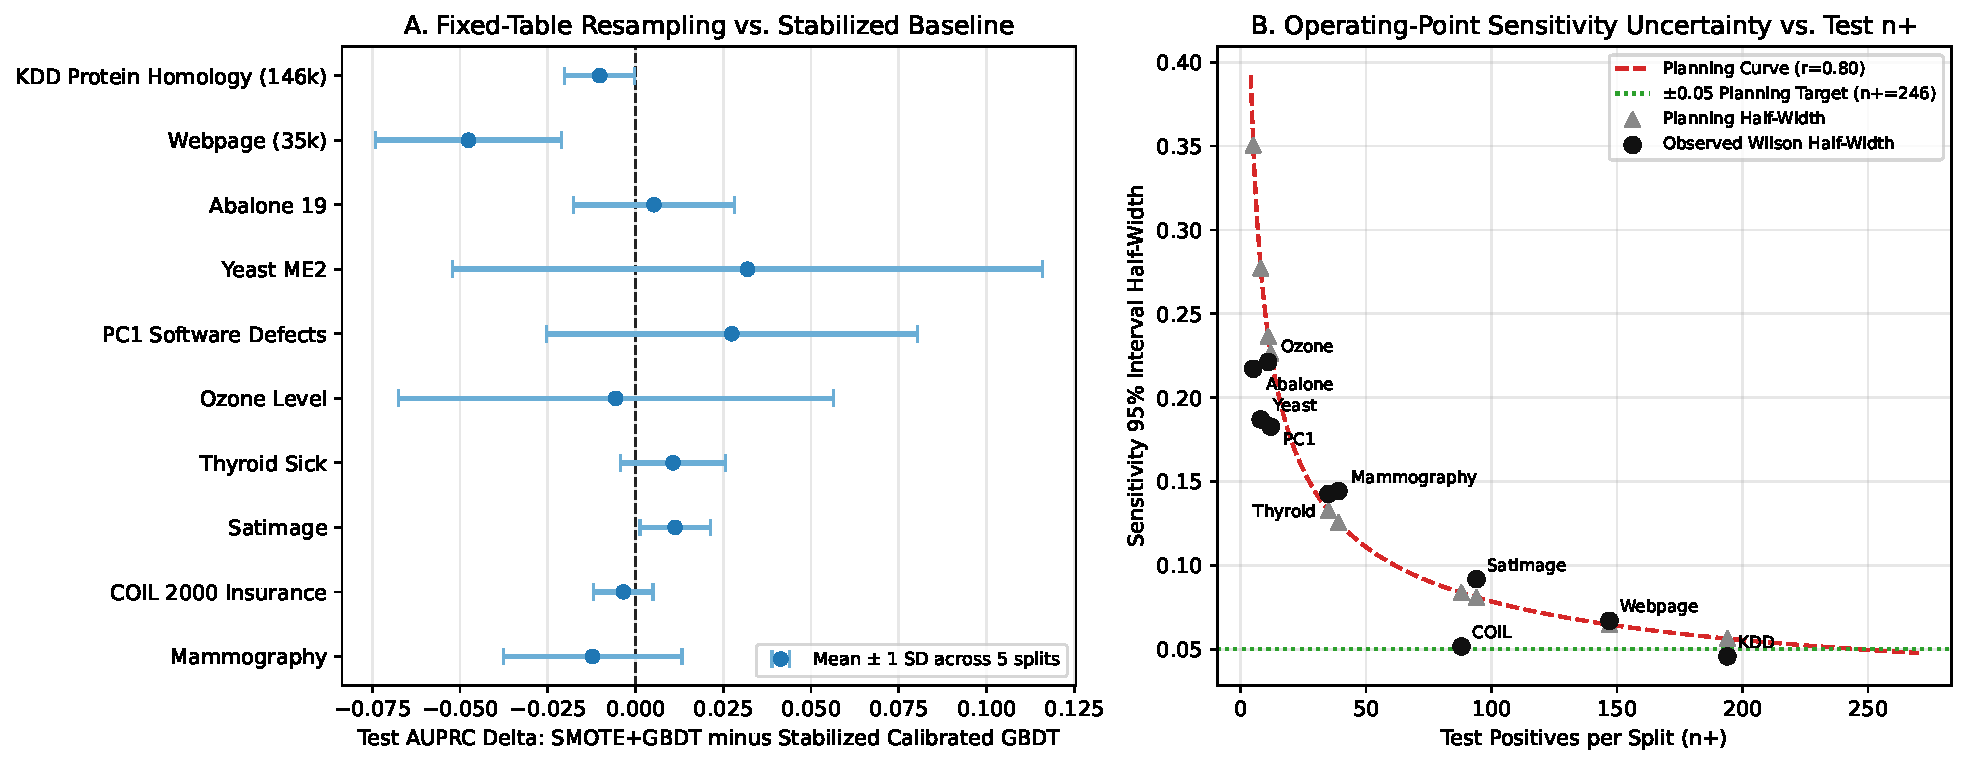
\includegraphics[width=0.96\textwidth]{fig1_tier1_saturation.pdf}
\caption{Fixed-table evaluation across 10 OpenML / \texttt{imbalanced-learn} datasets ($50$ splits). (A) Test AUPRC difference between SMOTE+GBDT and stabilized calibrated GBDT ($0/10$ significant gains). (B) Operating-point sensitivity uncertainty: prespecified planning half-widths ($r=0.80$) and observed Binomial Wilson $95\%$ half-widths versus held-out test positives per split ($n_+$).}
\label{fig:tier1}
\end{figure}

\subsection{Multi-Channel Discovery: Native Schemas vs.\ Injected-Proxy Stress Tests}
\label{sec:res_discovery}

To prevent synthetic proxy channels from inflating real-world claims, Table~\ref{tab:ablation} separates \textbf{Panel A (Native-Only Candidate Channels)} across all 9 cohorts ($45$ runs) from \textbf{Panel B (Injected Baseline-Echo Proxy Stress Tests)} across the 8 public cohorts ($40$ runs), while explicitly labeling dataset provenance: \texttt{real\_observational} (\texttt{UCI Diabetes 130-US}, $N=99,343$ eligible; \texttt{UCI Taiwan Credit}, $N=26,921$ eligible; \texttt{ULB Credit Card}, $N=284,807$ PCA blocks; \texttt{Scania APS}, $N=76,000$ anonymized truck counters and 10-bin histogram shape profiles; \texttt{Home Credit}, $N=307,511$ joined across 7 relational tables; \texttt{IEEE-CIS}, $N=590,540$ joined with the $24\%$-populated identity table), \texttt{privacy\_synthetic\_from\_real} (\texttt{NeurIPS BAF}, $N=1,000,000$), \texttt{synthetic\_physics} (\texttt{UCI AI4I}, $N=10,000$), and \texttt{synthetic\_simulator} (\texttt{Gate 0.5}, $N=12,000$).

\begin{table}[t]
\centering
\caption{Multi-channel discovery and downstream complexity evaluation ($5$ four-way splits per cohort). \textbf{Panel A (Primary Native-Only Suite, zero synthetic proxies):} Compares baseline $X_{\text{base}}$ GBDT (A0), $100\%$-row Global MI (A4), Unmatched Random-Pilot $\hat{G}_m$ (A4u), Stratified-Pilot $\hat{G}_m$ + Single GBDT (A5, Primary), Full-Cohort $100\%$-row $\hat{G}_m$ (A5f), Calibrated Hybrid Lattice (A7), and Unrestricted All-Native-Channels GBDT (Ref). \textbf{Panel B (Separate Injected-Proxy Stress Test):} Reports false proxy selection rates and resulting single-GBDT test AUPRC when noisy baseline-echo channels are added to the candidate pool.}
\label{tab:ablation}
\vspace{2pt}
\resizebox{\textwidth}{!}{%
\small
\setlength{\tabcolsep}{3.4pt}
\begin{tabular}{llcccccccc}
\toprule
\multicolumn{10}{l}{\textbf{Panel A: Primary Native-Only Candidate Channels (45 Splits; Mean Test AUPRC)}}\\
\midrule
\textbf{Cohort (Provenance)} & \textbf{Pilot} & \textbf{A0: Base} & \textbf{A4: GlobMI} & \textbf{A4u: Unm$\hat{G}_m$} & \textbf{A5: Strat$\hat{G}_m$} & \textbf{A5f: Full$\hat{G}_m$} & \textbf{A7: Lattice} & \textbf{Ref: All-Nat} & \textbf{Holm $p$} \\
 & \textbf{Used} & ($X_{\text{base}}$) & ($100\%$ rows) & (Pilot) & \textbf{(Primary)} & ($100\%$ rows) & (Selected) & (Unrestr.) & (A5 vs A0) \\
\midrule
Gate 0.5 (Sim.) & $20.5\%$ & $0.2104$ & $0.5415$ & $0.7964$ & $\mathbf{0.7964}$ & $0.7964$ & $0.8129$ & $0.7940$ & $\mathbf{0.00002}$ \\
UCI AI4I (Syn.\ Phys.) & $16.9\%$ & $0.3606$ & $0.7404$ & $0.7428$ & $\mathbf{0.7395}$ & $0.7404$ & $0.7339$ & $0.8702$ & $\mathbf{0.00299}$ \\
UCI Taiwan (Obs.) & $56.0\%$ & $0.2474$ & $0.4461$ & $0.4461$ & $\mathbf{0.4461}$ & $0.4461$ & $0.4505$ & $0.4506$ & $\mathbf{0.00025}$ \\
UCI Diabetes Adm.\ (Obs.) & $34.2\%$ & $0.1272$ & $0.2307$ & $0.2307$ & $\mathbf{0.2307}$ & $0.2307$ & $0.2307$ & $0.2338$ & $\mathbf{0.00233}$ \\
ULB Credit PCA (Obs.) & $1.2\%$ & $0.4821$ & $0.7428$ & $0.7428$ & $\mathbf{0.7541}$ & $0.7428$ & $0.7723$ & $0.7251$ & $\mathbf{0.01775}$ \\
Scania APS 76k (Obs.) & $9.0\%$ & $0.5260$ & $0.8499$ & $0.8655$ & $\mathbf{0.8662}$ & $0.8662$ & $0.8699$ & $0.8991$ & $\mathbf{0.00233}$ \\
Home Credit 7T (Obs.) & $40.4\%$ & $0.1678$ & $0.2489$ & $0.2557$ & $\mathbf{0.2557}$ & $0.2557$ & $0.2585$ & $0.2615$ & $\mathbf{0.00006}$ \\
IEEE-CIS 2T (Obs.) & $15.1\%$ & $0.1974$ & $0.4905$ & $0.4974$ & $\mathbf{0.4974}$ & $0.4974$ & $0.4983$ & $0.5078$ & $\mathbf{0.00123}$ \\
NeurIPS BAF 1M (Priv.\ Syn.) & $4.1\%$ & $0.0795$ & $0.1613$ & $0.1613$ & $\mathbf{0.1613}$ & $0.1613$ & $0.1688$ & $0.1643$ & $\mathbf{0.00299}$ \\
\midrule
\multicolumn{10}{l}{\textbf{Panel B: Separate Injected Baseline-Echo Proxy Stress Test (Large Multi-Table Cohorts Affected; 0\% Proxy Selection Elsewhere)}}\\
\midrule
\textbf{Cohort} & \textbf{Budget} & \textbf{GlobMI Proxy\%} & \textbf{UnmCC Proxy\%} & \textbf{PilotMI Proxy\%} & \textbf{A5 Proxy\%} & \textbf{GlobMI AP} & \textbf{A5 Strat$\hat{G}_m$ AP} & \textbf{NB $p$} & \textbf{Holm $p$} \\
\midrule
Home Credit 7T + Echoes & 3 of 7 & $33.3\%$ & $33.3\%$ & $33.3\%$ & $\mathbf{0.0\%}$ & $0.2454$ & $\mathbf{0.2557}$ & $\mathbf{0.0021}$ & $\mathbf{0.0168}$ \\
IEEE-CIS 2T + Echoes & 2 of 6 & $30.0\%$ & $10.0\%$ & $40.0\%$ & $\mathbf{0.0\%}$ & $0.4841$ & $\mathbf{0.4974}$ & $0.0562$ & $0.3370$ \\
NeurIPS BAF 1M + Echoes & 2 of 5 & $50.0\%$ & $50.0\%$ & $50.0\%$ & $\mathbf{0.0\%}$ & $0.1122$ & $\mathbf{0.1613}$ & $\mathbf{0.0111}$ & $0.0779$ \\
Other 5 Public Cohorts & 2 of $4$--$8$ & $0.0\%$ & $0.0\%$ & $0.0\%$ & $\mathbf{0.0\%}$ & \multicolumn{2}{c}{Matches Panel A native selection} & $\ge 0.166$ & $\ge 0.828$ \\
\bottomrule
\end{tabular}%
}
\end{table}

\begin{figure}[t]
\centering
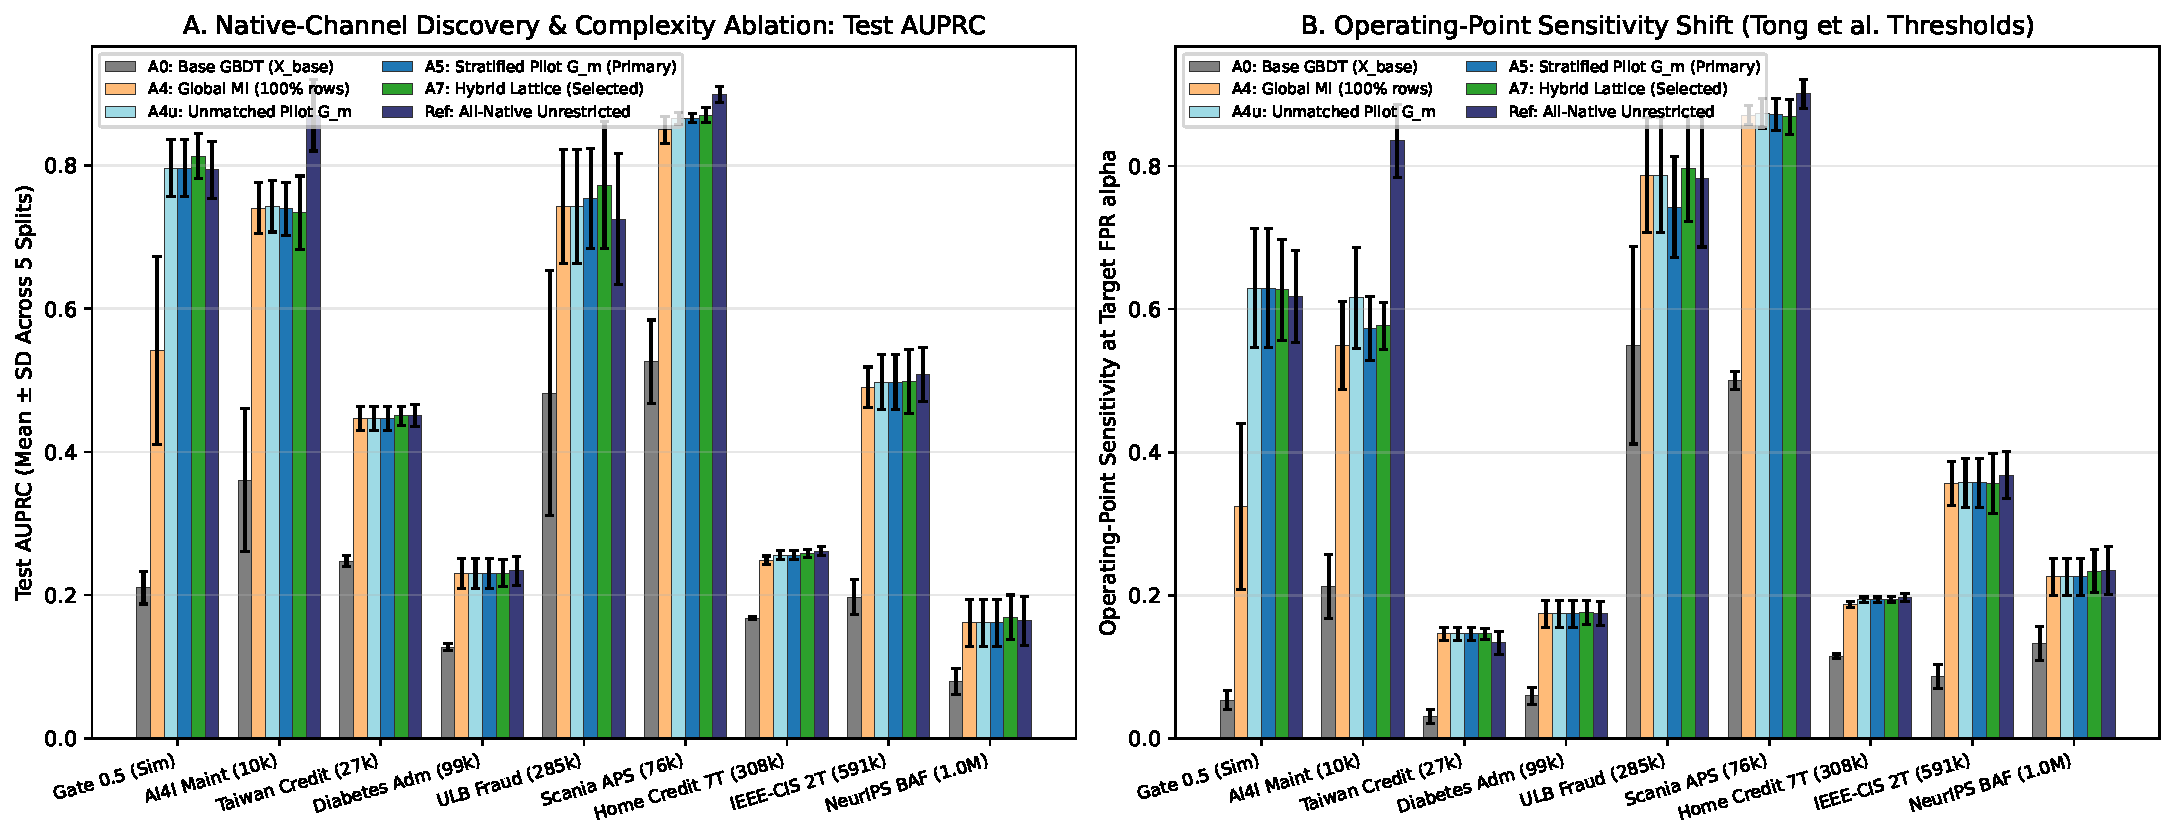
\includegraphics[width=0.96\textwidth]{fig2_ablation_ladder.pdf}
\caption{Native-channel discovery and downstream complexity ablations across all 9 cohorts ($45$ splits). (A) Test AUPRC (mean $\pm$ SD) comparing baseline $X_{\text{base}}$ (A0), $100\%$-row Global MI (A4), Unmatched-Pilot $\hat{G}_m$ (A4u), Primary Stratified-Pilot $\hat{G}_m$ + Single GBDT (A5), Hybrid Lattice (A7), and Unrestricted All-Native GBDT (Ref). (B) Corresponding operating-point sensitivity at Tong et al.\ $(\alpha,\delta=0.05)$-certified false-positive thresholds.}
\label{fig:ablation}
\end{figure}

Table~\ref{tab:ablation} and Figure~\ref{fig:ablation} establish five nuanced empirical conclusions:
\begin{enumerate}
  \item \textbf{Significant Gains Over $X_{\text{base}}$ With Certified Operating-Point FPR Control:} Across all $9/9$ native cohorts, primary Arm A5 ($\hat{G}_m$ + Single Calibrated GBDT) significantly improves over $X_{\text{base}}$ (A0) after conservative Nadeau--Bengio and Holm FWER adjustment on \emph{both} Test AUPRC (Holm $p \in [0.00002, 0.01775]$) and Tong et al.\ $(\alpha,\delta=0.05)$-certified Neyman--Pearson sensitivity (Holm $p \in [0.00013, 0.01807]$). Every split ($45/45$) satisfies $(1-\alpha)^m \le 0.05$, and realized test FPR remains strictly below target $\alpha$ on all 9 cohorts (e.g., $4.54\%$ at $\alpha=5\%$ on \texttt{Diabetes}; $0.46\%$ at $\alpha=0.5\%$ on \texttt{IEEE-CIS}; $0.13\%$ at $\alpha=0.2\%$ on \texttt{ULB}).
  \item \textbf{Pilot Efficiency Relative to Full-Cohort Conditional Discovery and Unrestricted Reference:} Measuring candidate channels only on the score-stratified pilot saves $44.0\%$ to $98.4\%$ of discovery channel accesses ($59.6\%$ to $98.4\%$ when $\pi < 10\%$, e.g., $3,834$ vs.\ $244,365$ channel-row accesses on \texttt{ULB} and $35,655$ vs.\ $858,000$ on \texttt{NeurIPS BAF}) while matching $100\%$-row Full-Cohort $\hat{G}_m$ (A5f) identically on $7/9$ cohorts, within $0.0009$ on \texttt{AI4I}, and $+0.0113$ higher on \texttt{ULB}. Relative to training an unrestricted GBDT on \emph{all} native channels (Ref), selecting $2$--$3$ channels recovers $96.3\%$--$103.9\%$ of all-native AUPRC on $8/9$ cohorts (trailing only on 3-channel synthetic \texttt{AI4I}, where the budget of $2$ omits the third distinct failure mode).
  \item \textbf{Admission-Time Clinical Case Study (\texttt{UCI Diabetes 130-US}):} Using strictly the 7 true admission-intake variables, A0 achieves $0.1272 \pm 0.0050$ AUPRC and $5.92\% \pm 1.15\%$ sensitivity at $\alpha=5\%$ (realized FPR $4.57\%$). Auditing the 6 candidate Stage-2 channels on a $34.2\%$ pilot ($112,644$ vs.\ $328,422$ discovery channel-row accesses, $65.7\%$ saved) consistently selects prior inpatient/ED/outpatient utilization plus discharge care-transition routing on $5/5$ patient-grouped splits, lifting single-GBDT A5 to $0.2307 \pm 0.0209$ AUPRC (Holm $p=0.00233$) and $17.38\% \pm 1.94\%$ sensitivity (Holm $p=0.00129$; realized FPR $4.54\%$), recovering $98.7\%$ of the all-6-native-channels GBDT ($0.2338$) while reducing downstream training/calibration accesses by $66.7\%$ ($169,060$ vs.\ $507,180$).
  \item \textbf{Where Conditional Gain Matters vs.\ Where Marginal MI Suffices:} On native schemas lacking strong baseline echoes (\texttt{Diabetes}, \texttt{Taiwan}, \texttt{AI4I}, \texttt{BAF}, \texttt{ULB}), $100\%$-row Global MI (A4) performs competitively with A5, whereas A5 improves over Global MI on confounded or relational native schemas (\texttt{Gate 0.5}: $0.7964$ vs.\ $0.5415$, $p_{\text{NB}}=0.011$; \texttt{Home Credit 7T}: $0.2557$ vs.\ $0.2489$, $p_{\text{NB}}=0.0029$; \texttt{Scania}: $0.8662$ vs.\ $0.8499$; \texttt{IEEE-CIS}: $0.4974$ vs.\ $0.4905$). Once exact HT weights and offset-anchored GBDT conditioning are applied, score-stratified pilot sampling (A5) provides a modest stability edge over unmatched random-pilot $\hat{G}_m$ (A4u) on ultra-rare \texttt{ULB} ($0.7541$ vs.\ $0.7428$) and \texttt{Scania} ($0.8662$ vs.\ $0.8655$) and ties elsewhere. Conversely, in the separate injected-proxy stress test (Panel B), Global MI, Unmatched CC MI, and Pilot MI suffer $30\%$--$50\%$ false proxy selection on the three large multi-table cohorts (\texttt{Home Credit} $0.2454$ vs.\ $0.2557$, Holm $p=0.0168$; \texttt{BAF} $0.1122$ vs.\ $0.1613$, $p_{\text{NB}}=0.0111$; \texttt{IEEE-CIS} $0.4841$ vs.\ $0.4974$), whereas A5 records $0.0\%$ false proxy selection across all $40$ stress runs. Moreover, clean $\hat{G}_m$ (A5) equals or outperforms the older composite heuristic \texttt{credo\_reg} on $9/9$ native cohorts (e.g., \texttt{ULB} $0.7541$ vs.\ $0.7291$, \texttt{BAF} $0.1613$ vs.\ $0.1504$).
  \item \textbf{Minimal Value of Downstream Ensemble Complexity:} Comparing Single-GBDT A5 against Calibrated Hybrid Lattice A7 shows small two-sided gains on only $2/9$ cohorts (\texttt{Home Credit} $+0.0028$, $p_2=0.025$; \texttt{NeurIPS BAF} $+0.0075$, $p_2=0.013$) and null differences on the remaining $7/9$ ($p_2 \ge 0.402$; exact tie $0.2307$ on \texttt{Diabetes}). Virtually all predictive lift comes from channel acquisition rather than post-selection lattice fusion.
\end{enumerate}

\subsection{Runtime Selective Acquisition Across Six Equal-Budget Policies}
\label{sec:res_routing}

Table~\ref{tab:foveation} and Figure~\ref{fig:foveation} evaluate all six equal-budget Stage-2 routing policies on the primary Single-GBDT A5 pipeline across all 9 native cohorts ($45$ splits). Confirming Proposition~\ref{prop:singleton}, Stage-1 Mondrian $\{1\}$ singletons occur on $3.7\%$--$22.1\%$ of test instances across all 9 cohorts yet achieve realized singleton PPV of only $3.8\%$--$38.8\%$ ($3.8\%$ on \texttt{NeurIPS BAF}, $10.1\%$ on \texttt{ULB}, $10.6\%$ on \texttt{IEEE-CIS}, $12.8\%$ on \texttt{Diabetes}). Because literal conformal ambiguity routing ($\{0,1\}$) leaves those $\{1\}$ singletons unverified at Stage 2, CREDO upper-tail acquisition outperforms literal $\{0,1\}$ routing on all $9/9$ cohorts (Holm $p \le 0.005$ on \texttt{Gate 0.5}, \texttt{Scania}, \texttt{Home Credit}, \texttt{IEEE-CIS}, and \texttt{NeurIPS BAF}), saving $24.3\%$--$79.0\%$ of simulated Stage-2 accesses while retaining $83.4\%$--$99.4\%$ of raw Stage-2 AUPRC and $76.3\%$--$98.4\%$ of incremental Stage-2 AUPRC gain over Stage 1 (at the explicit cost of leaving $2.3\%$--$24.3\%$ of true positives unqueried below the Stage-1 pruning gate).

\begin{table}[t]
\centering
\caption{Equal-budget runtime Stage-2 selective acquisition across 6 routing policies ($45$ native-channel splits). We report Stage-1 $\{1\}$ singleton PPV, simulated Stage-2 access savings, test AUPRC for Stage-1 Only, Random-$K$, Literal Conformal $\{0,1\}$, Uncertainty-$K$, VOI-$K$, Top-Risk-$K$, CREDO Upper-Tail, and $100\%$ Selected Stage-2, plus Incremental AP Gain Retention ($\text{IncRet}$), Unqueried Missed-Positive Fraction ($\text{UnqMP}$), Holm $p$ vs.\ Literal $\{0,1\}$, and two-sided $p_2$ vs.\ Top-Risk-$K$.}
\label{tab:foveation}
\vspace{2pt}
\resizebox{\textwidth}{!}{%
\small
\setlength{\tabcolsep}{2.8pt}
\begin{tabular}{lccccccccccccc}
\toprule
\textbf{Cohort} & \textbf{$\{1\}$} & \textbf{S2} & \textbf{S1} & \textbf{Rand} & \textbf{Lit} & \textbf{Unc} & \textbf{VOI} & \textbf{TopK} & \textbf{CREDO} & \textbf{100\%} & \textbf{IncRet /} & \textbf{Holm $p$} & $p_2$ \textbf{vs} \\
 & \textbf{PPV} & \textbf{Saved} & \textbf{Only} & $K$ & $\{0,1\}$ & $K$ & $K$ & $K$ & \textbf{UpTail} & \textbf{S2} & \textbf{UnqMP} & (vs $\{0,1\}$) & \textbf{TopK} \\
\midrule
Gate 0.5 & $15.4\%$ & $62.9\%$ & $0.2104$ & $0.4923$ & $0.4620$ & $0.6631$ & $0.6510$ & $0.6631$ & $\mathbf{0.6631}$ & $0.7964$ & $77.2\%$ / $22.5\%$ & $\mathbf{0.00190}$ & $1.000$ \\
UCI AI4I & $12.4\%$ & $77.1\%$ & $0.3606$ & $0.4343$ & $0.4424$ & $0.6534$ & $0.6323$ & $0.6534$ & $0.6517$ & $0.7395$ & $76.3\%$ / $24.3\%$ & $0.05323$ & $0.671$ \\
UCI Taiwan & $26.4\%$ & $34.6\%$ & $0.2474$ & $0.3937$ & $0.3917$ & $0.4179$ & $0.4073$ & $0.4179$ & $\mathbf{0.4179}$ & $0.4461$ & $85.8\%$ / $22.5\%$ & $0.13952$ & $1.000$ \\
UCI Diabetes & $12.8\%$ & $24.3\%$ & $0.1272$ & $0.2095$ & $0.2071$ & $0.2146$ & $\mathbf{0.2169}$ & $0.2146$ & $0.2146$ & $0.2307$ & $84.5\%$ / $19.7\%$ & $0.13952$ & $1.000$ \\
ULB Credit & $10.1\%$ & $79.0\%$ & $0.4821$ & $0.5347$ & $0.5415$ & $\mathbf{0.7510}$ & $0.7184$ & $\mathbf{0.7510}$ & $0.7357$ & $0.7541$ & $93.3\%$ / $6.3\%$ & $0.13952$ & $0.215$ \\
Scania APS & $38.8\%$ & $78.6\%$ & $0.5260$ & $0.6229$ & $0.6285$ & $\mathbf{0.8610}$ & $0.8262$ & $\mathbf{0.8610}$ & $0.8609$ & $0.8662$ & $98.4\%$ / $2.3\%$ & $\mathbf{0.00214}$ & $0.551$ \\
Home Credit & $16.3\%$ & $41.4\%$ & $0.1678$ & $0.2247$ & $0.2028$ & $0.2472$ & $0.2432$ & $0.2472$ & $\mathbf{0.2472}$ & $0.2557$ & $90.3\%$ / $20.2\%$ & $\mathbf{0.00214}$ & $1.000$ \\
IEEE-CIS & $10.6\%$ & $62.0\%$ & $0.1974$ & $0.3317$ & $0.2297$ & $0.4738$ & $0.4331$ & $0.4738$ & $\mathbf{0.4739}$ & $0.4974$ & $92.3\%$ / $22.7\%$ & $\mathbf{0.00059}$ & $0.358$ \\
NeurIPS BAF & $3.8\%$ & $61.9\%$ & $0.0795$ & $0.1108$ & $0.0844$ & $0.1568$ & $0.1425$ & $0.1568$ & $\mathbf{0.1568}$ & $0.1613$ & $94.6\%$ / $18.3\%$ & $\mathbf{0.00500}$ & $1.000$ \\
\bottomrule
\end{tabular}%
}
\end{table}

\begin{figure}[t]
\centering
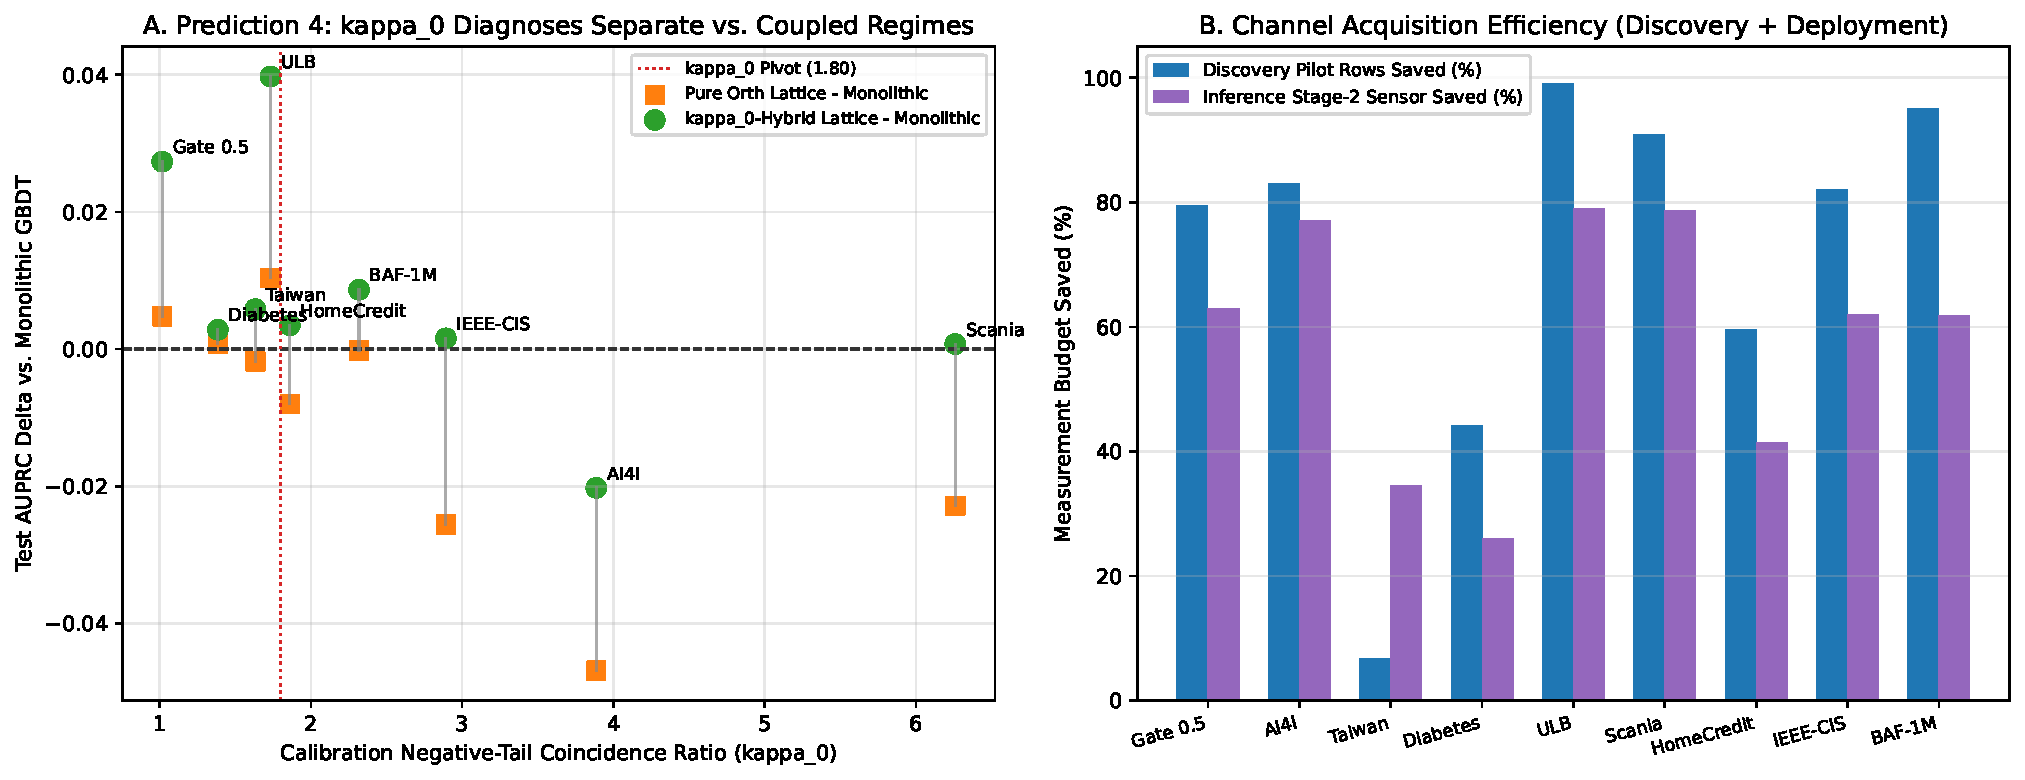
\includegraphics[width=0.96\textwidth]{fig3_kappa0_and_foveation.pdf}
\caption{Runtime selective acquisition and simulated access savings across 9 cohorts ($45$ splits). (A) Equal-budget test AUPRC across all 6 Stage-2 routing policies. (B) Simulated percentage of candidate channel-row accesses saved during training-time pilot discovery and deployment-time Stage-2 routing.}
\label{fig:foveation}
\end{figure}

\textbf{Critical Finding on Top-Risk-$K$ Equivalence:} Table~\ref{tab:foveation} reveals an essential operational insight that only emerges when \textbf{Top-Risk-$K$} and \textbf{Uncertainty-$K$} are included at equal budget $K$: across all 9 rare-event cohorts, \textbf{CREDO Upper-Tail} is statistically indistinguishable from \textbf{Top-Risk-$K$} ($p_2 \ge 0.215$; exact tie on $5/9$ cohorts, while Top-Risk-$K$ slightly leads on ultra-rare \texttt{ULB} at $0.7510$ vs.\ $0.7357$ and VOI-$K$ slightly leads on \texttt{Diabetes} at $0.2169$ vs.\ $0.2146$). Because Stage-1 baseline probabilities on these imbalanced cohorts almost never exceed $\max(q_{\text{target}}, 0.85) = 0.85$, the upper deficit cutoff rarely binds; consequently, Mondrian calibration here provides \textbf{principled query-budget sizing} ($K$ calibrated to $(\alpha_0, \alpha_1)$) rather than a superior instance ranking over Top-Risk-$K$ once $K$ is fixed.

\subsection{Controlled Adversarial and Failure-Mode Simulation Suite}
\label{sec:res_sims}

To establish exact boundary conditions where each discovery and routing rule succeeds or fails, Table~\ref{tab:sims} summarizes 7 synthetic adversarial regimes ($5$ seeds each $= 35$ runs):

\begin{table}[t]
\centering
\caption{Controlled 7-regime adversarial simulation suite ($5$ seeds per regime) probing conditional discovery, baseline misspecification, $m$-ratio sensitivity, VOI routing, unequal channel costs, and non-exchangeable temporal drift.}
\label{tab:sims}
\vspace{2pt}
\resizebox{\textwidth}{!}{%
\small
\setlength{\tabcolsep}{4.0pt}
\begin{tabular}{lllc}
\toprule
\textbf{Regime} & \textbf{Structural Mechanism Tested} & \textbf{Key Quantitative Outcome (Mean Across 5 Seeds)} & \textbf{Verdict} \\
\midrule
Sim 1: Pure Baseline Echo & $Z_{\text{echo}} = g(X_{\text{base}}) + \varepsilon$ vs.\ weaker $Z_{\text{orth}}$ & Global MI \& Pilot MI precision $0.0\%$; Full-$[X_{\text{base}},Z]$ $\hat{G}_m$ precision $\mathbf{100.0\%}$ & Rejects echo \\
Sim 2: Correlated Residual & $\operatorname{Corr}(Z, X_{\text{base}}) = 0.91$ with true residual signal & $\hat{G}_m$ selects informative correlated channel on $\mathbf{5/5}$ seeds ($100\%$) & Preserves signal \\
Sim 3: Pure Parity XOR & $Y$ depends on $\operatorname{sign}(X_1)\operatorname{sign}(Z_{\text{xor}})$; $I(Y;Z_{\text{xor}})=0$ & Global MI $0\%$; scalar-score $S(X_{\text{base}})$ CMI $0\%$; full-$[X_{\text{base}},Z]$ $\hat{G}_m$ $\mathbf{100\%}$ & Requires full $X_{\text{base}}$ \\
Sim 4: Underfit Stage-1 & Linear Stage-1 fit to quadratic $X_{\text{base}}^2$ + shadow $Z$ & Misspecified linear baseline fooled by $Z = X_1^2 + \varepsilon$ on $\mathbf{100\%}$ of seeds ($0\%$ under GBDT) & Failure boundary \\
Sim 5: Sparse Trigger $m$ & $\pi = 0.70\%$, sparse binary trigger ($n_{+,\text{train}} \approx 62$) & Top-1 hit \& test AUPRC rise from $80\%$ ($0.0366$) at $m \le 4$ to $\mathbf{100\%}$ ($\mathbf{0.0485}$) at $m \in \{8,16\}$ & Supports $m=8$ \\
Sim 6: Irreducible Top Pocket & Top $10\%$ irreducible ($p_1=0.86$); mid $10\%$ resolves $0/1$ & Top-Risk-$K$ ($0.8017$) \& CREDO ($0.8052$) fail; \textbf{VOI-$K$ ($\mathbf{0.8674}$)} \& \textbf{Lit $\{0,1\}$ ($\mathbf{0.8671}$)} win & Routing boundary \\
Sim 7: Unequal Cost \& Drift & Pair ($c=1+1$) vs.\ single ($c=2$); test covariate shift & $\hat{G}_m/c_m$ picks pair $100\%$ ($0.2256$ vs.\ $0.1315$); class-0 coverage drops $80.0\% \to \mathbf{62.4\%}$ ($-17.6\%$) & Drift vulnerability \\
\bottomrule
\end{tabular}%
}
\end{table}

Simulations~3, 4, 6, and 7 make the paper's methodological boundaries explicit: (i) conditioning solely on a compressed scalar baseline score $S(X_{\text{base}})$ fails completely ($0\%$) on pure parity/XOR interactions that full-$[X_{\text{base}}, Z_m]$ offset-anchored GBDTs recover ($100\%$, Sim~3); (ii) conditional discovery is only as strong as the Stage-1 nuisance learner---underfitting $X_{\text{base}}$ causes nonlinear baseline shadows to masquerade as novel signal ($100\%$ false selection, Sim~4); (iii) when the highest-risk Stage-1 pocket already lies safely above the decision threshold with irreducible Stage-2 noise while an intermediate-risk pocket contains resolvable ambiguity, upper-tail and top-risk routing waste queries ($0.8052$ and $0.8017$ AUPRC; net utility $389.4$), whereas \textbf{VOI-$K$} ($0.8674$; net utility $422.3$) and \textbf{Literal $\{0,1\}$} ($0.8671$) recover full Stage-2 performance (Sim~6); and (iv) unweighted Mondrian conformal thresholds lose $17.6$ percentage points of nominal class-0 coverage under post-calibration covariate shift, motivating importance-weighted conformal extensions \citep{barber2023conformal} in non-stationary streams (Sim~7).

\section{Discussion, Limitations, and Conclusions}

Our reconstructed theoretical and empirical analysis reframes imbalanced tabular prediction around budgeted information acquisition while stripping away unsupported universal claims:
\begin{enumerate}
  \item \textbf{Stabilized Baselines Before Resampling:} Across 10 fixed-table benchmarks, once leaf Newton steps are bounded (\texttt{max\_delta\_step}$=1.0$) and probabilities are Platt-calibrated on natural prevalence, standard resampling and undersampled ensembles yield zero statistically detectable AUPRC improvements and widen calibration error unless recalibrated. On small cohorts ($n_+ \le 12$), reporting exact Wilson $95\%$ sensitivity intervals prevents mistaking Binomial sampling noise for algorithmic progress.
  \item \textbf{Stratified-Pilot Conditional Discovery + Simple Downstream Models:} Evaluating candidate channels on a known-probability baseline-stratified case-cohort pilot via Horvitz--Thompson offset-anchored conditional log-likelihood gain $\hat{G}_m$ cuts pilot channel accesses by $44\%$--$98\%$, matches full-cohort conditional selection within $0.0009$ AUPRC on $8/9$ cohorts, immunizes multi-table discovery against baseline echoes ($0\%$ vs.\ $30\%$--$50\%$ false proxy selection), and achieves nearly all downstream predictive gains with a single calibrated GBDT.
  \item \textbf{When Conformal Routing Helps---and When Simple Risk or VOI Routing Is Better:} Under low prevalence, positive conformal singletons $\{1\}$ routinely suffer low PPV ($3.8\%$--$38.8\%$), explaining why querying upper-tail candidates achieves higher mean AUPRC than literal $\{0,1\}$ ambiguity routing across $9/9$ cohorts (Holm $p \le 0.005$ on $5/9$). When Stage-1 risk rarely exceeds $q_{\text{target}}$, however, upper-tail conformal routing reduces to Top-Risk-$K$ ordering with conformal budget sizing; and when top-risk pockets carry low expected loss reduction relative to mid-risk pockets, decision-focused VOI-$K$ routing is strictly preferable.
\end{enumerate}

\textbf{Limitations:} Four limitations bound our conclusions. First, all Stage-2 acquisitions on public cohorts are retrospective masked-column simulations on pre-collected datasets \citep{vonkleist2025evaluation}; in live clinical workflows, diagnostic ordering patterns can induce missing-not-at-random ascertainment shifts requiring prospective validation. Second, as Simulation~4 demonstrates, $\hat{G}_m$ relies on expressive Stage-1 conditioning and can select nonlinear baseline functions if Stage 1 is misspecified. Third, greedy per-channel ranking $\hat{G}_m/c_m$ can over-select redundant pairs among Stage-2 channels themselves unless sequential conditional updates $\hat{G}_{m \mid \mathcal{S}}$ are computed. Fourth, standard Mondrian conformal thresholds require exchangeability and suffer coverage drift under non-stationarity (Simulation~7), where weighted conformal methods \citep{barber2023conformal} should be adopted.

\appendix
\section{Mathematical Proofs}
\label{app:proofs}

\begin{proof}[Proof of Lemma~\ref{lem:prior_shift}]
Under class-conditional invariance $\tilde{\mathbb{P}}(X_{\text{base}} \in A \mid Y=y) = \mathbb{P}(X_{\text{base}} \in A \mid Y=y)$ for $y \in \{0,1\}$, Bayes' rule gives posterior odds $\tilde{\eta}(x)/[1-\tilde{\eta}(x)] = [\tilde{\pi}/(1-\tilde{\pi})] L(x) = \gamma\, \eta_{\text{base}}(x)/[1-\eta_{\text{base}}(x)]$ with $\gamma = \tilde{\pi}(1-\pi)/[\pi(1-\tilde{\pi})] > 0$, yielding $\tilde{\eta}(x) = \gamma \eta_{\text{base}}(x)/[\gamma \eta_{\text{base}}(x) + 1 - \eta_{\text{base}}(x)]$. Since $d\tilde{\eta}/d\eta_{\text{base}} = \gamma / [\gamma \eta_{\text{base}} + 1 - \eta_{\text{base}}]^2 > 0$ on $(0,1)$, superlevel sets $\{x : \tilde{\eta}(x) > \tilde{\tau}\}$ coincide with $\{x : \eta_{\text{base}}(x) > \tau\}$ for $\tau = g_\gamma^{-1}(\tilde{\tau})$, preserving population ROC and PR curves \citep{elkan2001foundations}. Under natural prevalence $\pi$, $\mathbb{P}(Y=1 \mid \tilde{\eta}(X_{\text{base}})=s) = g_\gamma^{-1}(s) \ne s$ for $\gamma \ne 1$ whenever $s \in (0,1)$. Finally, achieving posterior probability $\ge q_{\text{target}}$ requires posterior log-odds $\ge \operatorname{logit}(q_{\text{target}})$, leaving non-negative log-odds gap $D_q(x) = \max\{0, \operatorname{logit}(q_{\text{target}}) - \operatorname{logit}(\eta_{\text{base}}(x))\}$.
\end{proof}

\begin{proof}[Proof of Lemma~\ref{lem:ht_cmi}]
For part (1), conditioning on $X_{\text{base}}=x$ and using $\mathbb{P}(Y=1 \mid X_{\text{base}}=x) = \eta_{\text{base}}(x)$ yields $\mathbb{E}[\ell(Y, \eta_{\text{base}}(X_{\text{base}})) \mid X_{\text{base}}=x] = -\eta_{\text{base}}(x)\log \eta_{\text{base}}(x) - [1-\eta_{\text{base}}(x)]\log[1-\eta_{\text{base}}(x)] = H(Y \mid X_{\text{base}}=x)$. Conditioning on $(X_{\text{base}}=x, Z_m=z)$ similarly yields $\mathbb{E}[\ell(Y, \eta_m(X_{\text{base}}, Z_m)) \mid X_{\text{base}}=x, Z_m=z] = H(Y \mid X_{\text{base}}=x, Z_m=z)$. Taking expectations over $(X_{\text{base}}, Z_m)$ by the law of iterated expectations gives $\mathbb{E}[g_m(X_{\text{base}}, Z_m, Y)] = H(Y \mid X_{\text{base}}) - H(Y \mid X_{\text{base}}, Z_m) = I(Y; Z_m \mid X_{\text{base}}) \ge 0$, which vanishes if and only if $Y \perp Z_m \mid X_{\text{base}}$ \citep{covert2023learning,gadgil2024estimating}. For part (2), let $I_i \in \{0,1\}$ indicate pilot inclusion given $\mathcal{D}_{\text{train}}$. By construction, $\mathbb{E}[I_i \mid \mathcal{D}_{\text{train}}] = 1$ for $Y_i = 1$ ($w_i = 1$) and $\mathbb{E}[I_i \mid \mathcal{D}_{\text{train}}] = n_{0,b}/N_{0,b} > 0$ for $Y_i = 0$ in stratum $b$ ($w_i = N_{0,b}/n_{0,b}$). Linearity of expectation gives $\mathbb{E}_{\mathcal{P}}[\frac{1}{N}\sum_{i=1}^N I_i w_i \psi_i \mid \mathcal{D}_{\text{train}}] = \frac{1}{N}\sum_{i=1}^N \mathbb{E}[I_i \mid \mathcal{D}_{\text{train}}] w_i \psi_i = \frac{1}{N}\sum_{i=1}^N \psi_i$.
\end{proof}

\begin{proof}[Proof of Proposition~\ref{prop:singleton}]
By Bayes' rule on $\mathcal{S}_{\{1\}}$, $\operatorname{PPV}(\mathcal{S}_{\{1\}}) = \pi \gamma_1 / [\pi \gamma_1 + (1-\pi)\gamma_0]$. Since $0 \notin \mathcal{C}_1(x)$ iff $\hat{p}_1(x) > \hat{q}_{1-\alpha_0}^{(0)}$, Mondrian validity on calibration negatives implies $\gamma_0 \le \alpha_0$ in expectation while imposing no lower bound on $\alpha_0 - \gamma_0$; rearranging $\operatorname{PPV}(\mathcal{S}_{\{1\}}) < q_{\text{target}}$ gives $\pi < q_{\text{target}}\gamma_0 / \allowbreak [q_{\text{target}}\gamma_0 + (1-q_{\text{target}})\gamma_1]$. For the $(\alpha,\delta)$ Neyman--Pearson threshold \citep{tong2018neyman}, let $S_1,\dots,S_m \stackrel{\text{i.i.d.}}{\sim} F_0$ be negative calibration scores and let $R(s) = \mathbb{P}_{X \sim F_0}(S(X) > s)$ denote the strict-inequality population false-positive rate. Define $s_\alpha = \inf\{s \in \mathbb{R} : R(s) \le \alpha\}$; by right-continuity of $1 - R(s)$, $R(s_\alpha) \le \alpha$. Under the strict rule $S(X) > S_{(r)}$, the event $\{R(S_{(r)}) > \alpha\}$ implies $S_{(r)} < s_\alpha$, which holds only if at least $r$ of the $m$ negative calibration scores satisfy $S_i < s_\alpha$. Since $\mathbb{P}_{F_0}(S_i < s_\alpha) \le 1 - \alpha$ even under arbitrary point masses (e.g., if $S \equiv 0.20$, then $s_\alpha = 0.20$, $S_{(r)} = 0.20$, and $R(S_{(r)}) = \mathbb{P}(0.20 > 0.20) = 0 \le \alpha$), Binomial tail dominance yields
\[
  \mathbb{P}\!\left(R(S_{(r)}) > \alpha\right) \le \sum_{j=r}^{m} \binom{m}{j}(1-\alpha)^j \alpha^{m-j} \le \delta. \qedhere
\]
\end{proof}

\section*{Author Contributions}

Conceptualization, methodology, software, validation, formal statistical analysis, investigation, writing---original draft, and writing---review and editing: W.A.S. The author has read and agreed to the published version of the manuscript.

\section*{Funding}

This research received no external grant funding. Computational and agentic research platform access was supported by the Google Antigravity for Science program.

\section*{Institutional Review Board and Informed Consent Statement}

Ethical review and approval and patient informed consent were not required for this study under 45 CFR 46.104(d)(4) because all analyses were conducted exclusively on publicly available, fully de-identified, and anonymized benchmark datasets with zero human subject recruitment, intervention, or private health information access.

\section*{Data and Code Availability}

{\raggedright All source code (\texttt{imboreceipt} Python package), deterministic benchmark runners, unit and counterexample regression test suites (\texttt{31/31} passing tests), SHA-256 split and eligibility manifests, and reconstructed campaign JSON receipts (\texttt{results/reconstructed/}) supporting the findings of this study are publicly available under the MIT License at \url{https://github.com/deesatzed/imboreceipt} and in the accompanying reproducibility archive (\texttt{credo\_reproducibility\_code.zip}). The 19 evaluated benchmark cohorts comprise 18 external public datasets accessible through the UCI Machine Learning Repository (\url{https://archive.ics.uci.edu/dataset/296}, \url{https://archive.ics.uci.edu/dataset/350}, \url{https://archive.ics.uci.edu/dataset/601}), OpenML (\url{https://www.openml.org/d/310}, \url{https://www.openml.org/d/1068}, \url{https://www.openml.org/d/1597}), Kaggle public competition archives (\texttt{Home Credit Default Risk} and \texttt{IEEE-CIS Fraud Detection}), and the NeurIPS Bank Account Fraud archive (\url{https://doi.org/10.48550/arXiv.2211.13358}), plus 1 deterministic synthetic multi-mechanism simulator (\texttt{Gate 0.5}) included in the open-source package.\par}

\section*{Acknowledgments}

Computational and agentic research platform access was supported by the Google Antigravity for Science program.

\section*{Competing Interests}

The author declares no competing financial or commercial interests.

\bibliographystyle{plainnat}
\bibliography{references}

\end{document}
